\documentclass{article}
\usepackage{amsmath}
\usepackage{graphicx}


\title{\LaTeX}
\date{}
\begin{document}
\underline{4.3 \c{C}ifte\c{s}lik  \hspace{6cm}}\\
\textit{Gerek Ko\c{s}ul :}\\
E\u{g}er \c{c}izge d\"{u}zlemsel de\u{g}ilse, bir alt\c{c}izgesi\\
Kuratowski \c{c}izgelerinden birine k\"{o}kte\c{s} olacakt{\i}r.\\
\"{O}yleyse, gerek ko\c{s}ulu tan{\i}tlamak i\c{c}in her iki \\
Kuratowski \c{c}izgesinin de \c{c}ifte\c{s}i olmad{\i}\u{g}{\i}n{\i} \\
g\"{o}stermemiz yeterlidir.
$\c{S}ekil\quad 4.3.4a$ da gösterilen $K_1$ \c{c}izgesine ili\c{s}kin \\
t-\c{c}evre matrisi,\\
$\bar{B}_tl$ = \bordermatrix{
      ~ & 1 & 2 & 3 & 4 & 5 & 6 & 7 & 8 & 9 & 10  \cr
     1 & 1 & 0 & 0 & 0 & 0 & 0 & 1 & 1 & 0 & 0  \cr
     2 & 0 & 1 & 0 & 0 & 0 & 0 & 0 & 1 & 1 & 0  \cr
     3 & 0 & 0 & 1 & 0 & 0 & 0 & 0 & 0 & 1 & 1   \cr
     4 & 0 & 0 & 0 & 1 & 1 & 0 & 0 & 1 & 0 & 1  \cr
     5 & 0 & 0 & 0 & 0 & 1 & 0 & 1 & 0 & 1 & 0 \cr
     6 & 0 & 0 & 0 & 0 & 0 & 1 & 1 & 0 & 0 & 1 \cr
}\\

\begin{figure}[h]
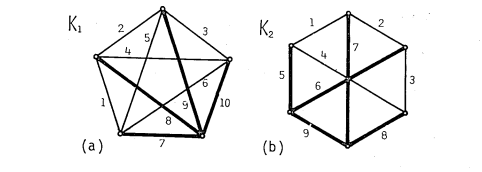
\includegraphics{images/image1.png}
\end{figure}

$\c{S}ekil 4.3.4$ Whitney teoreminde gerek ko\c{s}ulun tan{\i}t{\i}.
\end{document}
